\documentclass[letterpaper, 12pt]{article}

%%%%%%%%%%%%%%%%%%%%%%%%%%%%%
% DEFINITIONS
% Change those informations
% If you need umlauts you have to escape them, e.g. for an ü you have to write \"u
\gdef\mytitle{Laborprotokoll}
\gdef\mythema{DezSys05 - Java Security}

\gdef\mysubject{Systemtechnik-Labor}
\gdef\mycourse{5BHIT 2015/16, Gruppe Z}
\gdef\myauthor{Michael Weinberger}

\gdef\myversion{0.1}
\gdef\mybegin{15. Januar 2016}
\gdef\myfinish{???}

\gdef\mygrade{Note:}
\gdef\myteacher{Betreuer: Micheler}
%
%%%%%%%%%%%%%%%%%%%%%%%%%%%%%

\input special/preamble.tex

\let\tempsection\section
\renewcommand\section[1]{\vspace{-0.3cm}\tempsection{#1}\vspace{-0.3cm}}
\WithSuffix\newcommand\section*[1]{\tempsection*{#1}}

\let\tempsubsection\subsection
\renewcommand\subsection[1]{\vspace{0cm}\tempsubsection{#1}\vspace{0cm}}

\let\tempsubsubsection\subsubsection
\renewcommand\subsubsection[1]{\vspace{0cm}\tempsubsubsection{#1}\vspace{0cm}}

\linespread{0.94}

\lhead{\mysubject}
\chead{}
\rhead{\bfseries\mythema}
\lfoot{\mycourse}
\cfoot{\thepage}
% Creative Commons license BY
% http://creativecommons.org/licenses/?lang=de
\rfoot{\ccby\hspace{2mm}\myauthor}
\renewcommand{\headrulewidth}{0.4pt}
\renewcommand{\footrulewidth}{0.4pt}

\begin{document}
\parindent 0pt
\parskip 6pt

\pagenumbering{Roman} 
%!TEX root=../laborprotokoll.tex

\begin{titlepage}

	\begin{figure}[!h]
		\begin{flushright}
			
\includegraphics[width=0.3\linewidth]{images/jdIT_tgm.png}
		\end{flushright}
	\end{figure}

	\vspace{2.5cm} 

	{\begin{center} \bfseries\huge
			\rule{17.5cm}{0.1mm}  
			\\[5mm]
			\mytitle\\[5mm]
			\mythema\\
			\rule{17.5cm}{0.1mm}  
	\end{center}}

	{\begin{flushright} \bfseries\Large
			\vspace{2cm}
			\mysubject\\
			\mycourse\\[10mm]
			\myauthor\\[10mm]
	\end{flushright}}

	{\begin{table}[!h] \bfseries\normalsize
		\begin{tabularx}{\textwidth}{lXr @{\hspace{0mm}}}
			&& Version \myversion\\
			\mygrade && Begonnen am \mybegin\\
			\myteacher && Beendet am \myfinish\\
		\end{tabularx}
	\end{table}}

\end{titlepage}


\clearpage
\thispagestyle{empty}
\tableofcontents

\newpage
\pagenumbering{arabic}
\pagestyle{fancy}

%\vspace{-0.5cm}
\section{Einführung}
Diese Übung zeigt die Anwendung von Verschlüsselung in Java.
\subsection{Ziele}
Das Ziel dieser Übung ist die symmetrische und asymmetrische Verschluesselung in Java umzusetzen. Dabei soll ein Service mit einem Client einen sicheren Kommunikationskanal aufbauen und im Anschluss verschlüsselte Nachrichten austauschen. Ebenso soll die Verwendung eines Namensdienstes zum Speichern von Informationen (hier PublicKey) verwendet werden. \\
Die Kommunikation zwischen Client und Service soll mit Hilfe einer Übertragungsmethode (IPC, RPC, Java RMI, JMS, etc) aus dem letzten umgesetzt werden.
\subsection{Voraussetzungen}
\begin{itemize}
	\item Grundlagen Verzeichnisdienst
	\item Administration eines LDAP Dienstes
	\item Grundlagen der JNDI API für eine JAVA Implementierung
	\item Grundlagen Verschluesselung (symmetrisch, asymmetrisch)
	\item Einfuehrung in Java Security JCA (Cipher, KeyPairGenerator, KeyFactory)
	\item Kommunikation in Java (IPC, RPC, Java RMI, JMS)
	\item Verwendung einer virtuellen Instanz für den Betrieb des Verzeichnisdienstes
\end{itemize}

\subsection{Aufgabenstellung}
Mit Hilfe der zur Verfuegung gestellten VM wird ein vorkonfiguriertes LDAP Service zur Verfügung gestellt. Dieser Verzeichnisdienst soll verwendet werden, um den PublicKey von einem Service zu veröffentlichen. Der PublicKey wird beim Start des Services erzeugt und im LDAP Verzeichnis abgespeichert. Wenn der Client das Service nutzen will, so muss zunaechst der PublicKey des Services aus dem Verzeichnis gelesen werden. Dieser PublicKey wird dazu verwendet, um den symmetrischen Schluessel des Clients zu verschlüsseln und im Anschluss an das Service zu senden. \\
Das Service empfängt den verschlüsselten symmetrischen Schluessel und entschlüsselt diesen mit dem PrivateKey. Nun kann eine Nachricht verschlüsselt mit dem symmetrischen Schlüssel vom Service zum Client gesendet werden. \\
Der Client empfängt die verschlüsselte Nachricht und entschlüsselt diese mit dem symmetrischen Schlüssel. Die Nachricht wird zuletzt zur Kontrolle ausgegeben. \newpage
Die folgende Grafik soll den Vorgang verdeutlichen: 
\begin{figure}[!h]
	\begin{center}
		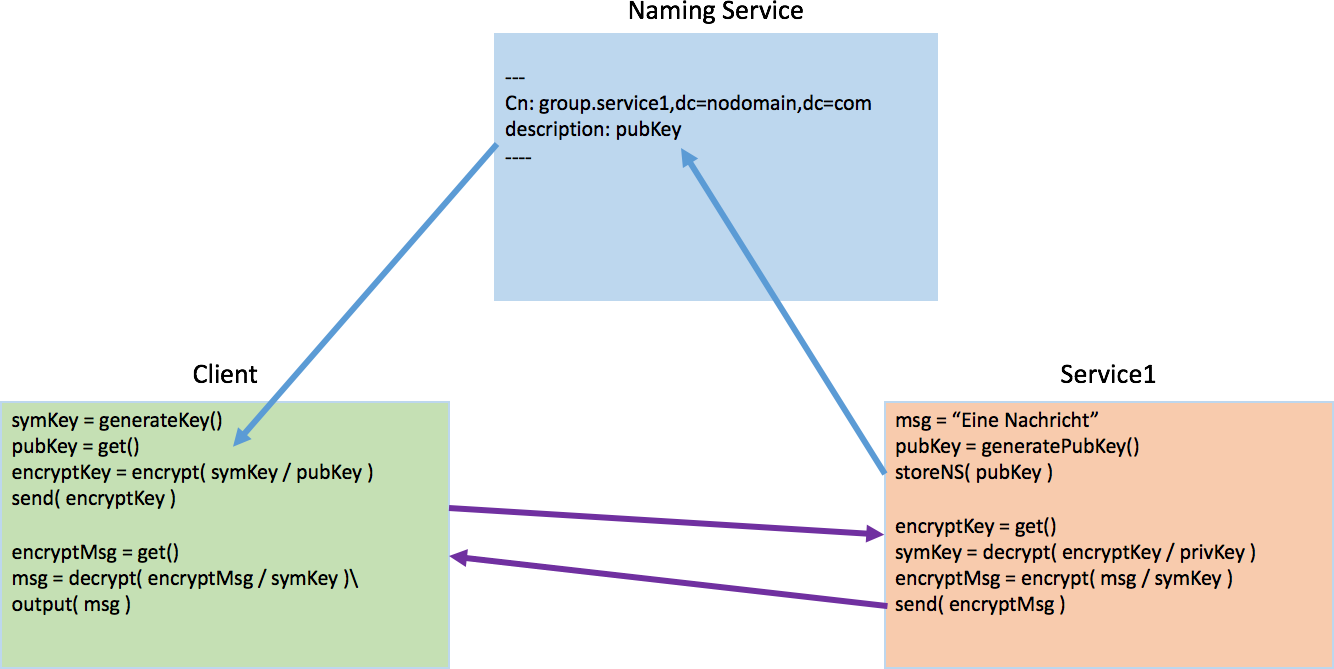
\includegraphics[width=1\linewidth]{images/dezsys05_java_security_demo1}
		\caption{Angabe}
		\label{Angabe}
	\end{center}
\end{figure}

\subsection{Bewertung}
\textit{16 Punkte}
\begin{itemize}
	\item asymmetrische Verschluesselung (4 Punkte)
	\item symmetrische Verschluesselung (4 Punkte)
	\item Kommunikation in Java (3 Punkte)
	\item Verwendung eines Naming Service, JNDI (3 Punkte)
	\item Protokoll (2 Punkte)
\end{itemize}

\newpage

\section{asdf}

\newpage

\bibliographystyle{unsrt}
\bibliography{references}
\lstlistoflistings
\listoffigures

\end{document}
